% Introduction to R for Teaching / Advising


\documentclass{beamer}
\usetheme{CambridgeUS}
\usepackage{array}


\title{Using R to Analyze and Visualize Education Data}

\author{Jared Knowles}
% - Use the \inst{?} command only if the authors have different
%   affiliation.

\institute[DPI] % (optional, but mostly needed)
{
  Policy Research Advisor\\
  Wisconsin Department of Public Instruction
}
\date[R Bootcamp] % (optional)
{\today / R Bootcamp}


% If you have a file called "university-logo-filename.xxx", where xxx
% is a graphic format that can be processed by latex or pdflatex,
% resp., then you can add a logo as follows:

%\pgfdeclareimage[height=0.5cm]{university-logo}{OHSU_H_4C_POS_RGB}
%\logo{\pgfuseimage{university-logo}}

\usepackage{Sweave}
\usepackage{dcolumn, multirow}
\usepackage{epsfig,graphicx}
\usepackage{verbatim, rotating, paralist,hyperref}
\usepackage{float}
\graphicspath{{./img/}} %additional graphics directory




% If you wish to uncover everything in a step-wise fashion, uncomment
% the following command:

%\beamerdefaultoverlayspecification{<+->}


\AtBeginDocument{ 
\DefineVerbatimEnvironment{Sinput}{Verbatim} {xleftmargin=2em,fontsize= 
\footnotesize} 
\DefineVerbatimEnvironment{Soutput}{Verbatim}{xleftmargin=2em,fontsize= 
\footnotesize} 
\DefineVerbatimEnvironment{Scode}{Verbatim}{xleftmargin=2em,fontsize= 
\footnotesize} 
}

\begin{document}



\begin{frame}
  \titlepage
\end{frame}


\begin{frame}{Outline}
  \tableofcontents
\end{frame}


%% Some intro content about R

\section{Introduction to R?}

\begin{frame}
\frametitle{\textbf{R}}
  \begin{itemize}
  \item R is an Open Source (and freely available) environment for statistical computinga nd graphics
  \item Available for Windows, Mac OS X, and Linux
  \item R is being actively developed with two major releases per year and dozens of releases of add on packages
  \item R can be extended with 'packages' that contain data, code, and documentation to add new functionality
  \end{itemize}
\end{frame}

\subsection{Why Use R?}
\begin{frame}
\frametitle{R Advantages}
\begin{itemize}
  \item R is a common tool among data experts at major universities
  \item No need to go through procurement, R can be installed in any environment on any machine and used with no licensing or agreements needed
  \item R source code is very readable to increase transparency of processes
  \item R code is easily borrowed from and shared with others
  \item R is incredibly flexible and can be adapted to specific local needs
  \item R is under incredibly active development, improving greatly, and supported wildly by both professional and academic developers
  \end{itemize}
\end{frame}

\begin{frame}
\frametitle{R Advantages Continued}
\begin{itemize}
  \item R is platform agnostic--Linux, Mac, PC, server, desktop, etc.
  \item R can output results in a variety of formats
  \item R can build routines straight out of a database for common and universal reporting
\end{itemize}
\end{frame}

\begin{frame}
\frametitle{R Can Compliment}
\begin{itemize}
\item R plays nicely with data from Stata, SPSS, SAS and others
\item R can check work, produce output, visualize results from other programs
\item R can do bleeding edge analysis that aren't available in proprietary packages yet
\item R is becoming more prevalent in undergraduate statistics courses
\end{itemize}
\end{frame}


\begin{frame}
\frametitle{R Popularity}
\vspace{-.1in}
\begin{center}
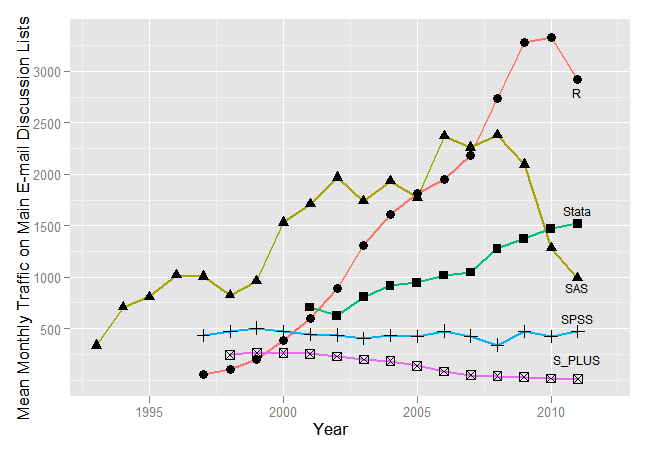
\includegraphics[height=.78\paperheight]{rlistserv}
\end{center}
\end{frame}


\begin{frame}
\frametitle{R Popularity II}
\vspace{-.1in}
\begin{center}
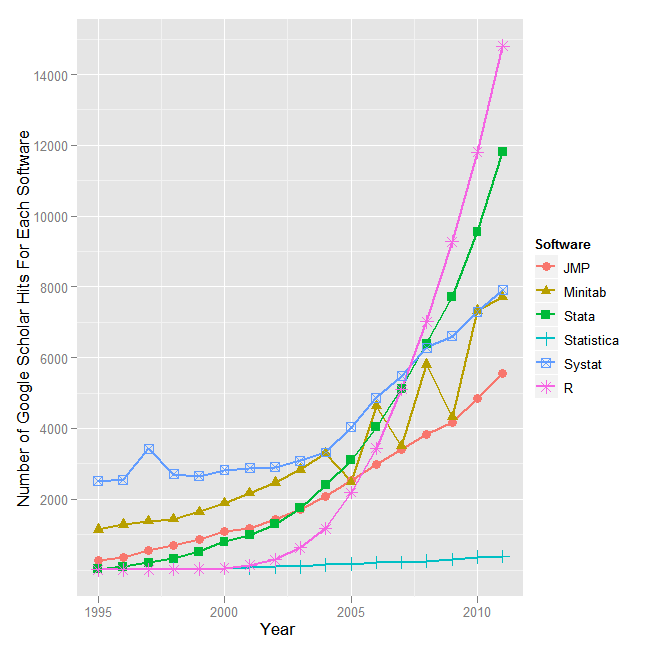
\includegraphics[height=.77\paperheight]{googlescholar}
\end{center}
\end{frame}


\begin{frame}
\frametitle{R Popularity III}
\vspace{-.1in}
\begin{center}
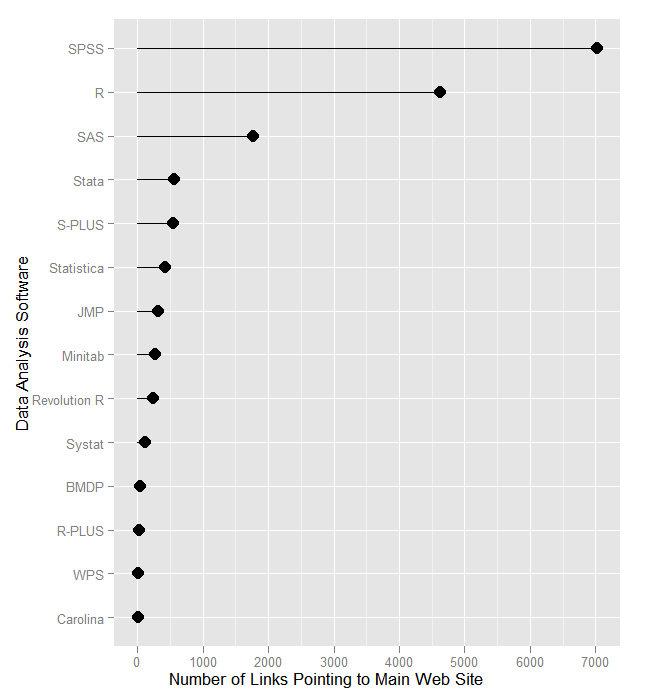
\includegraphics[height=.78\paperheight]{sitelinks}
\end{center}
\footnotesize Data from Robert Muenchen at https://sites.google.com/site/r4statistics/popularity 2010-2012
\end{frame}

\subsection{R Setup}
\begin{frame}
\frametitle{Windows}
\begin{itemize}
  \item Setting up R on Windows XP is straightforward. On Windows 7 or Vista you may need to run in administrator mode to install extensions.
  \item Standard R interface in Windows is pretty ugly. 
\end{itemize}

\begin{center}
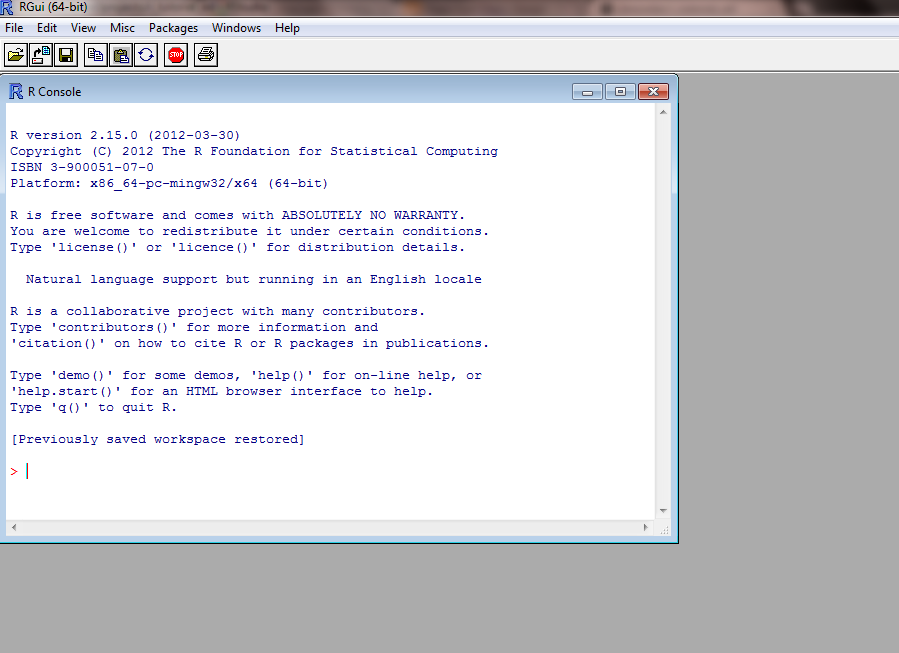
\includegraphics[height=.4\paperheight,width=.6\textwidth]{rgui}
\end{center}
\end{frame}

\begin{frame}
\frametitle{Using an IDE To Make Things Easier}
\begin{center}
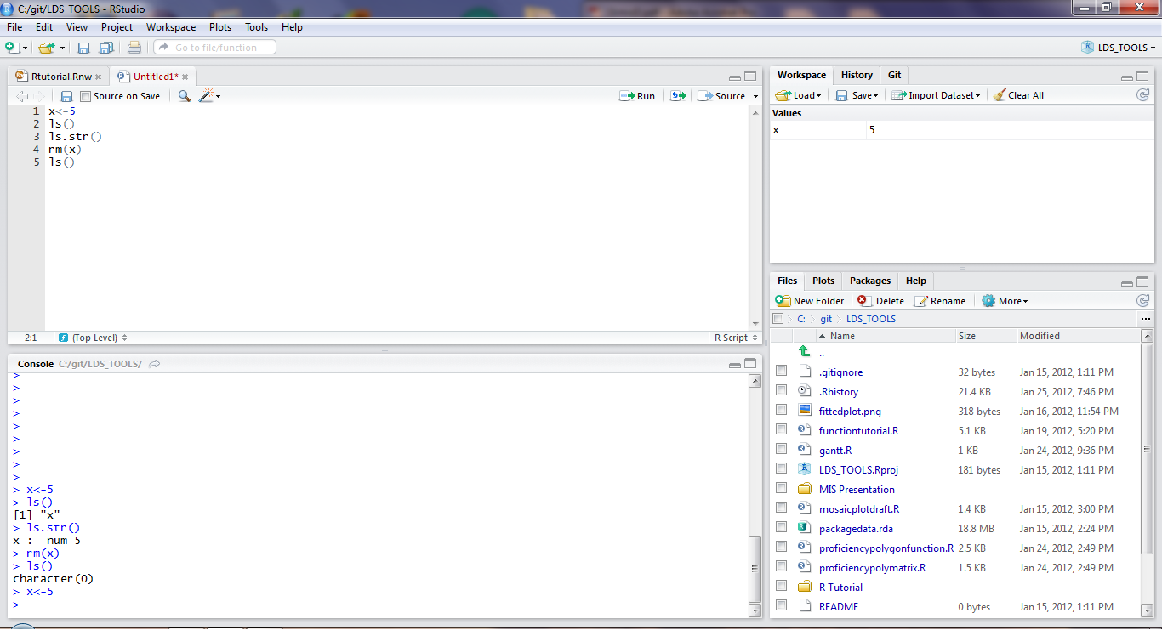
\includegraphics[height=.76\paperheight,width=.9\textwidth]{workspacescreen}
\end{center}
\end{frame}


\section{Using R}
\subsection{The Basics}
\begin{frame}[containsverbatim]
\frametitle{R as a Calculator}
\begin{Schunk}
\begin{Sinput}
> 2+2 # add numbers
\end{Sinput}
\begin{Soutput}
[1] 4
\end{Soutput}
\begin{Sinput}
> 2*pi #multiply by a constant
\end{Sinput}
\begin{Soutput}
[1] 6.283185
\end{Soutput}
\begin{Sinput}
> 7+runif(1,min=0,max=1) #add a random variable
\end{Sinput}
\begin{Soutput}
[1] 7.59793
\end{Soutput}
\begin{Sinput}
> 4^4 # powers
\end{Sinput}
\begin{Soutput}
[1] 256
\end{Soutput}
\begin{Sinput}
> sqrt(4^4) # functions
\end{Sinput}
\begin{Soutput}
[1] 16
\end{Soutput}
\end{Schunk}
\end{frame}

\begin{frame}[containsverbatim]
\frametitle{Using the Workspace}
  \begin{itemize}
  \item To do more we need to learn how to manipulate the 'workspace'.
  \item This includes all the scalars, vectors, datasets, and functions stored in memory.
  \item All R objects are stored in the memory of the computer, limiting the available space for calculation to the size of the RAM on your machine.
  \item R makes organizing the workspace easy.
  \end{itemize}
\begin{Schunk}
\begin{Sinput}
> x<-5 #store a variable with <-
> x    #print the variable
\end{Sinput}
\begin{Soutput}
[1] 5
\end{Soutput}
\begin{Sinput}
> z<-3 
> ls() #list all variables
\end{Sinput}
\begin{Soutput}
[1] "x" "z"
\end{Soutput}
\begin{Sinput}
> ls.str() #list and describe variables
\end{Sinput}
\begin{Soutput}
x :  num 5
z :  num 3
\end{Soutput}
\begin{Sinput}
> rm(x)    # delete a variable
> ls()
\end{Sinput}
\begin{Soutput}
[1] "z"
\end{Soutput}
\end{Schunk}
\end{frame}

\section{Getting Data In}
\begin{frame}[containsverbatim]
\frametitle{Reading Data}
\begin{itemize}
  \item To read data in we have to tell R where it currently is on the filesystem
  \item Then we have to tell it where to look for the dataset and how to read it
  \item CSV files are simplest for beginning use cases, but R is flexible
\end{itemize}
\begin{Schunk}
\begin{Sinput}
> # Set working directory to the tutorial director
> # In RStudio can do this in "Tools" tab
> setwd('~/r_tutorial_ed')
> #Load some data
> df<-read.csv('data/smalldata.csv')
> # Note if we don't assign data to 'df'
> # R just prints contents of table
\end{Sinput}
\end{Schunk}
\end{frame}

\begin{frame}[containsverbatim]
\frametitle{Objects}
\begin{itemize}
  \item Everything in R is an object--even functions
  \item Objects can be manipulated many ways
  \item A common example is applying the `summary' function to a variety of object types and seeing how it adapts
\end{itemize}
\begin{Schunk}
\begin{Sinput}
> summary(df[,28:31]) #summary look at df object
\end{Sinput}
\begin{Soutput}
   schoollow          readSS          mathSS     
 Min.   :0.0000   Min.   :251.5   Min.   :210.2  
 1st Qu.:0.0000   1st Qu.:430.0   1st Qu.:418.3  
 Median :0.0000   Median :495.3   Median :480.1  
 Mean   :0.2422   Mean   :496.2   Mean   :483.4  
 3rd Qu.:0.0000   3rd Qu.:562.5   3rd Qu.:543.2  
 Max.   :1.0000   Max.   :833.2   Max.   :828.4  
        proflvl    
 advanced   : 788  
 basic      : 523  
 below basic: 210  
 proficient :1179  
\end{Soutput}
\begin{Sinput}
> summary(df$readSS) #summary of a single column
\end{Sinput}
\begin{Soutput}
   Min. 1st Qu.  Median    Mean 3rd Qu.    Max. 
  251.5   430.0   495.3   496.2   562.5   833.2 
\end{Soutput}
\end{Schunk}
\end{frame}


\section{Handling Data in R}

\section{Cleaning and Merging Data in R}

\section{Analytics}

\section{Visualizations}

\section{Outputting Results}

\section{Writing Functions, Sharing Code}







\end{document}
